\chapter{Группирование и оконные функции}
\section{Написание запросов для группировки данных}


\begin{lstlisting}[label=lst:funcReturn, language=sql]
	SELECT shipperid,
	COUNT(*) AS numorders,
	COUNT(shippeddate) AS shippedorders,
	MIN(shippeddate) AS firstshipdate,
	MAX(shippeddate) AS lastshipdate,
	SUM(val) AS totalvalue
   FROM Sales.OrderValues
   GROUP BY shipperid; 
\end{lstlisting}

Обратите внимание на разницу между результатами функций COUNT(shippeddate) и
COUNT(*). Первая игнорирует значения NULL в столбце shippeddate, и поэтому дает
количество заказов меньшее или равное количеству заказов, полученных во второй
функции.

Используя общие функции наборов, можно работать с отдельными вхождениями,
указывая предложение DISTINCT перед выражением, как в следующем примере: 


\begin{lstlisting}[label=lst:funcReturn, language=sql]
	SELECT shipperid, COUNT(DISTINCT shippeddate) AS numshippingdates
	FROM Sales.Orders
	GROUP BY shipperid;
\end{lstlisting}

Опция DISTINCT доступна не только в функции COUNT, но также в других общих
функциях наборов. Однако, как правило, она используется с функцией COUNT.

\section{Работа с несколькими наборами группирования}


Язык T-SQL поддерживает три выражения, которые позволяют задавать несколько наборов группирования: GROUPING SETS, CUBE и
ROLLUP. Они используются в предложении GROUP BY.

\subsection{GROUPING SETS}

Выражение GROUPING SETS можно использовать для создания списка наборов группирования, которые требуется определить в запросе. Следующий запрос определяет четыре набора группирования:

\begin{lstlisting}[label=lst:funcReturn, language=sql]
SELECT shipperid, YEAR(shippeddate) AS shipyear, COUNT(*) AS numorders
FROM Sales.Orders
WHERE shippeddate IS NOT NULL
GROUP BY GROUPING SETS
(
( shipperid, YEAR(shippeddate)),
	( shipperid ),
	( YEAR(shippeddate) ),
	( )
); 
\end{lstlisting}


\begin{figure}[h!]
	\begin{center}
		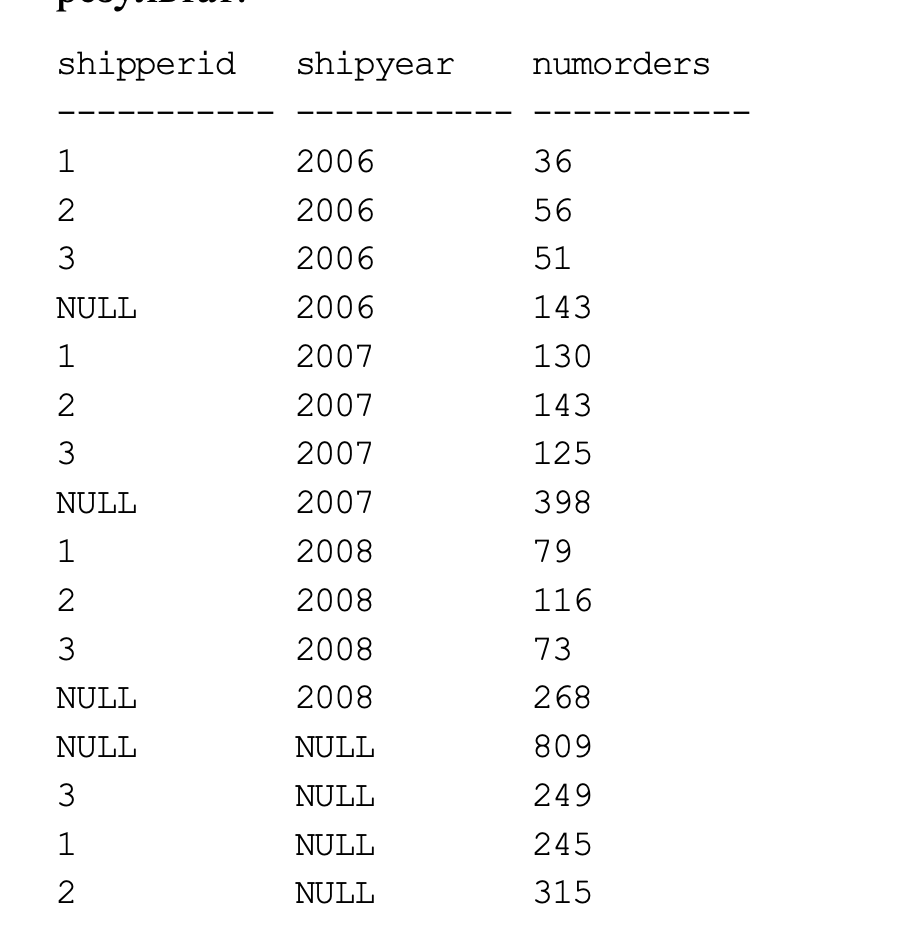
\includegraphics[width=0.6\textwidth]{img/res11.png}
	\end{center}
	\captionsetup{justification=centering}
\end{figure}

\subsection{CUBE}
Выражение CUBE принимает список выражений на вход и определяет
все возможные наборы группирования, которые могут быть сгенерированы из входов, включая пустой набор группирования. Например, следующий запрос является
логическим эквивалентом предыдущего запроса, использовавшего выражение
GROUPING SETS. 

\begin{lstlisting}[label=lst:funcReturn, language=sql]
SELECT shipperid, YEAR(shippeddate) AS shipyear, COUNT(*) AS numorders
FROM Sales.Orders
GROUP BY CUBE(shipperid, YEAR(shippeddate));
\end{lstlisting}

Выражение CUBE определяет все четыре возможных набора группирования из двух
входов: 

\begin{enumerate}
	\item (shipperid, YEAR(shippeddate)). 
	\item (shipperid). 
	\item (YEAR(shippeddate)). 
	\item ( ). 
\end{enumerate}

\subsection{ROLLUP}


Выражение ROLLUP также представляет собой сокращенный вариант выражения
GROUPING SETS, но оно используется, когда существует иерархическая структура,
сформированная входными элементами. В таком случае только поднабор возможных наборов группирования представляет реальный интерес.
Рассмотрим, например, иерархию местоположений, созданную в этом заказе элементами shipcountry,
shipregion и shipcity. Имеет смысл свертывать данные только в одном направлении, производя статистические вычисления для следующих наборов группирования: 

\begin{enumerate}
	\item (shipcountry, shipregion, shipcity). 
	\item (shipcountry, shipregion). 
	\item (shipcountry).  
	\item ( ). 
\end{enumerate}

Другие наборы группирования просто не интересны. Например, хотя одно и то же
название города может появиться в разных местах в мире, нет смысла агрегировать
все вхождения этого названия — независимо от региона и страны. 

\begin{lstlisting}[label=lst:funcReturn, language=sql]
	SELECT shipcountry, shipregion, shipcity, COUNT(*) AS numorders
	FROM Sales.Orders
	GROUP BY ROLLUP(shipcountry, shipregion, shipcity); 
\end{lstlisting}

\begin{figure}[h!]
	\begin{center}
		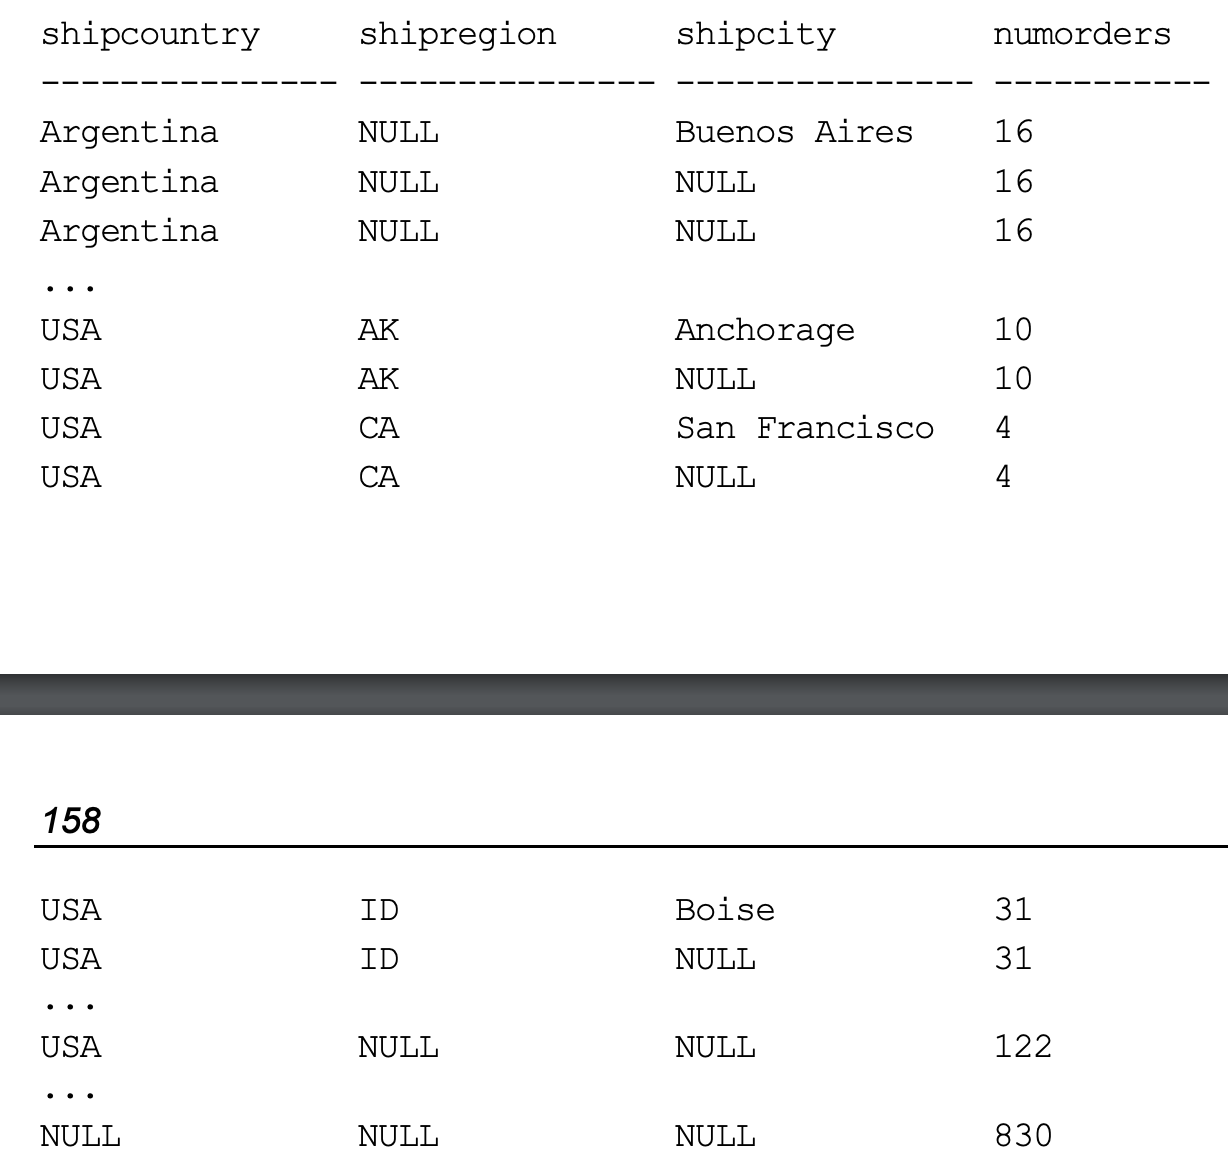
\includegraphics[width=0.8\textwidth]{img/res12.png}
	\end{center}
	\captionsetup{justification=centering}
\end{figure}

Проблема возникает при определении строк,
связанных с одиночным набором группирования, когда сгруппированный столбец
разрешает значения NULL — как в случае со столбцом shipregion. Как объяснить,
представляет ли значение NULL в результате замещающее значение (означающее
"все регионы") или исходное значение NULL из таблицы (означающее "неприменимый регион")? В языке T-SQL имеются две функции, позволяющие решить эту
проблему: GROUPING и GROUPING\_ID. 

\subsection{GROUPING, GROUPING\_ID}

Функция GROUPING принимает единственный элемент на вход и возвращает 0, если
этот элемент входит в состав набора группирования, и 1 — когда не входит в него.
Следующий запрос демонстрирует использование функции GROUPING: 

\begin{lstlisting}[label=lst:funcReturn, language=sql]
	SELECT
	shipcountry, GROUPING(shipcountry) AS grpcountry,
	shipregion , GROUPING(shipregion) AS grpregion,
	shipcity , GROUPING(shipcity) AS grpcity,
   COUNT(*) AS numorders
   FROM Sales.Orders
   GROUP BY ROLLUP(shipcountry, shipregion, shipcity); 
\end{lstlisting}

\begin{figure}[h!]
	\begin{center}
		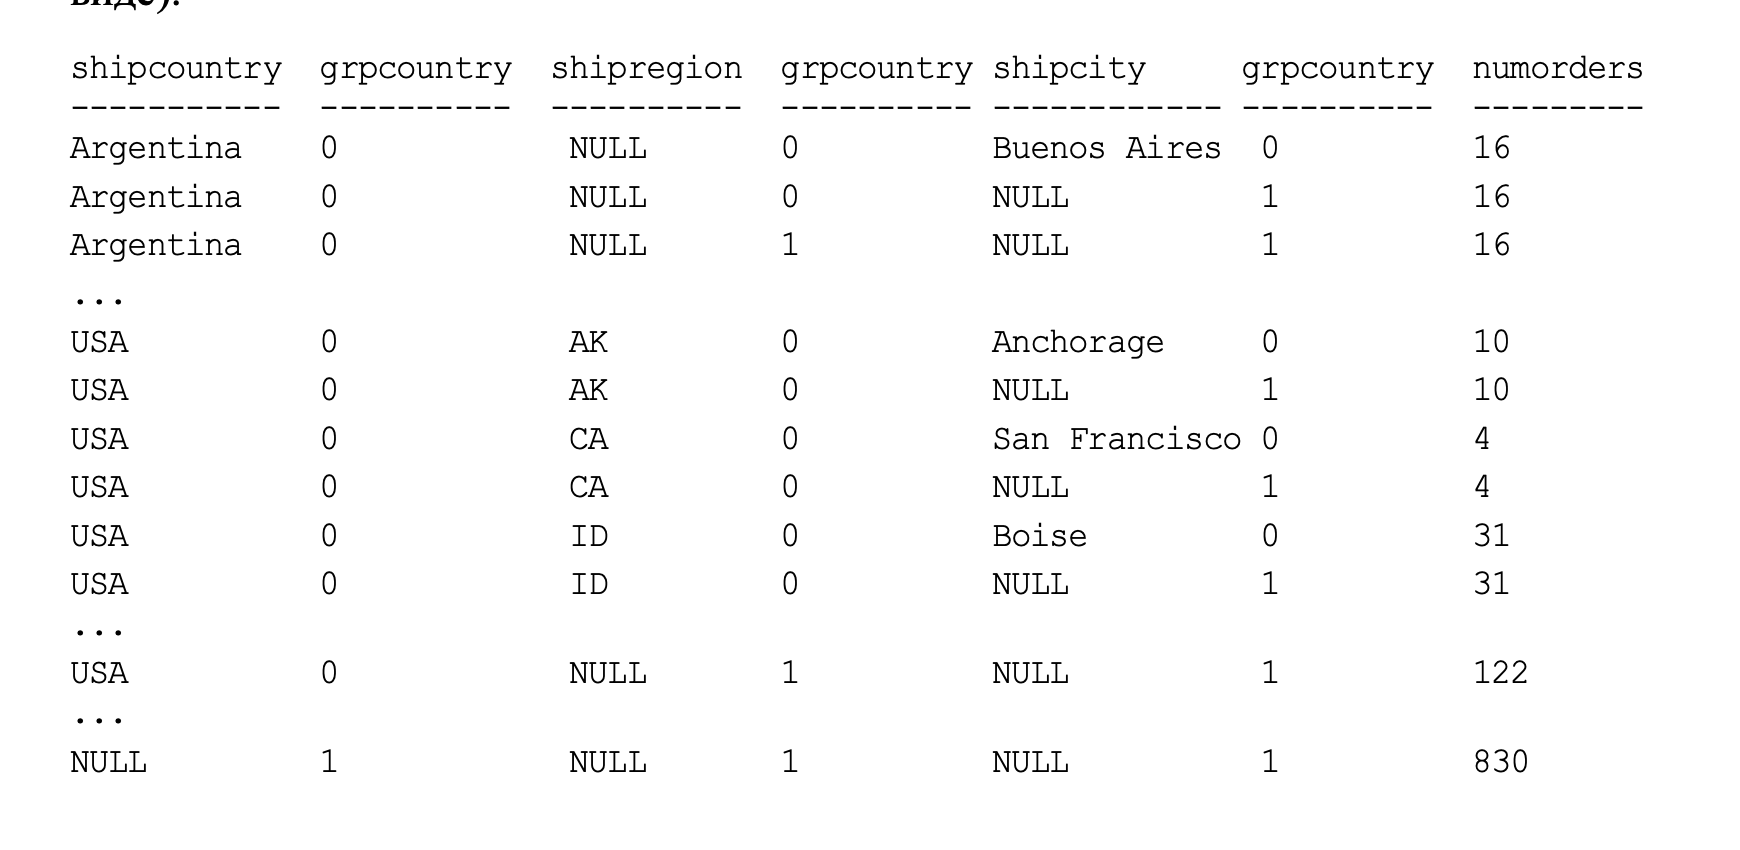
\includegraphics[width=0.8\textwidth]{img/res13.png}
	\end{center}
	\captionsetup{justification=centering}
\end{figure}	


Другая функция, которую можно использовать для определения наборов группирования — GROUPING\_ID. Она принимает на вход список сгруппированных столбцов и
возвращает целое число, представляющее битовую карту. Самый правый бит представляет самое правое входное значение. Этот бит равен 0, когда соответствующий
элемент является частью набора группирования, и 1 — в противном случае.

\begin{lstlisting}[label=lst:funcReturn, language=sql]
	SELECT GROUPING_ID(shipcountry, shipregion, shipcity) AS grp_id,
	shipcountry, shipregion, shipcity,
	COUNT(*) AS numorders
   FROM Sales.Orders
   GROUP BY ROLLUP( shipcountry, shipregion, shipcity ); 
\end{lstlisting}	



\begin{figure}[h!]
	\begin{center}
		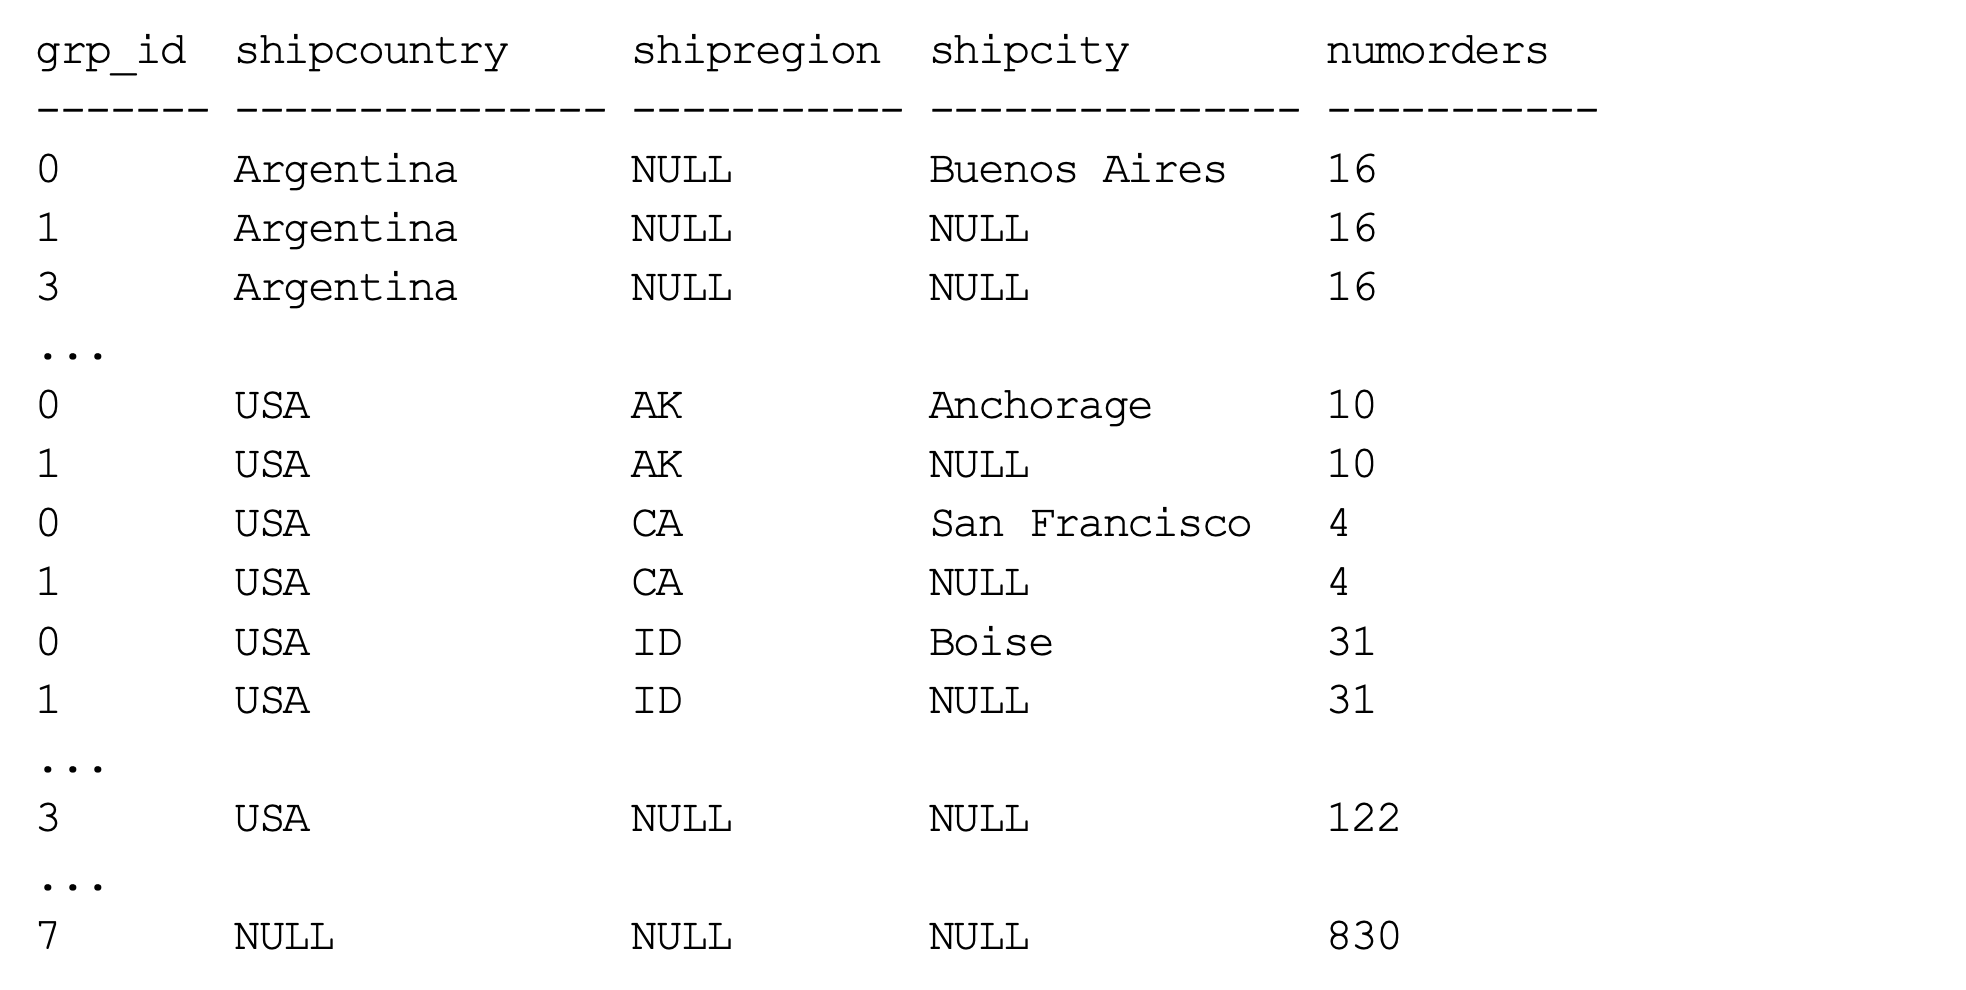
\includegraphics[width=0.8\textwidth]{img/res14.png}
	\end{center}
	\captionsetup{justification=centering}
\end{figure}	


\begin{figure}[h!]
	\begin{center}
		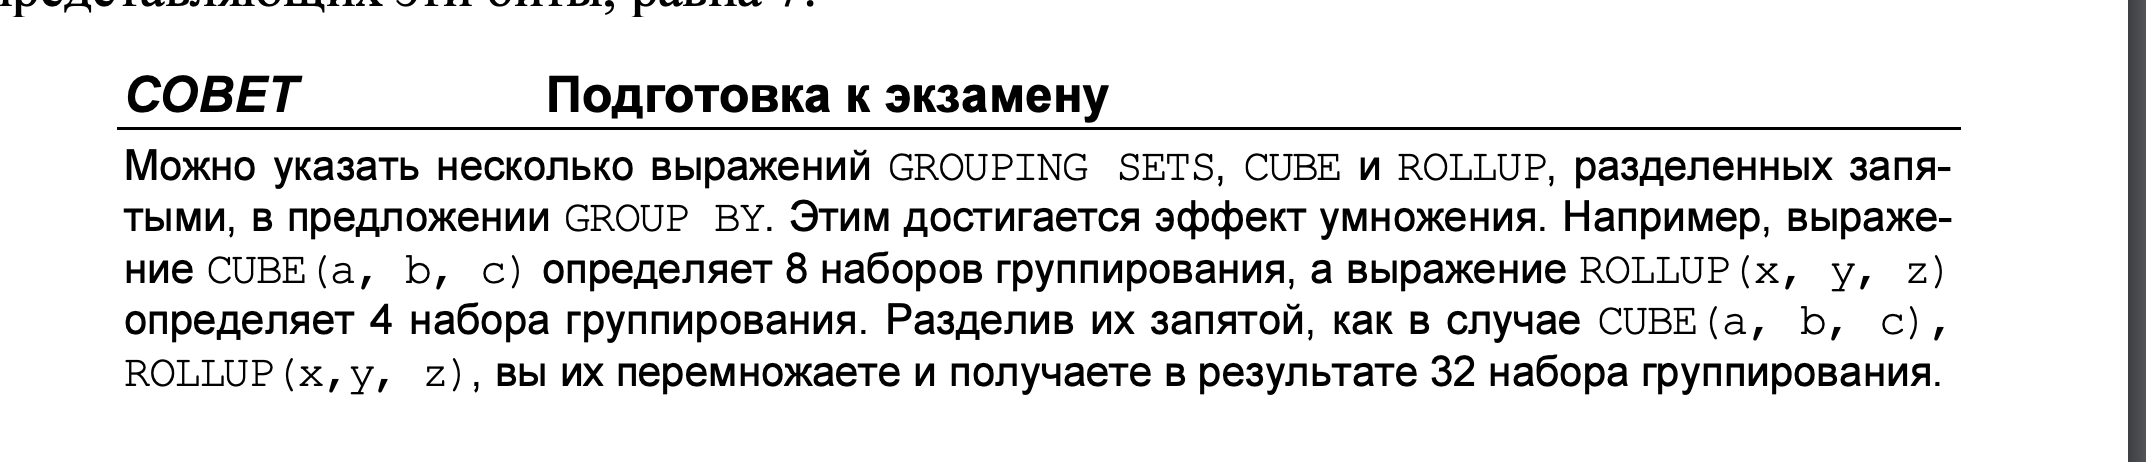
\includegraphics[width=0.8\textwidth]{img/advice9.png}
	\end{center}
	\captionsetup{justification=centering}
\end{figure}	


\begin{figure}[h!]
	\begin{center}
		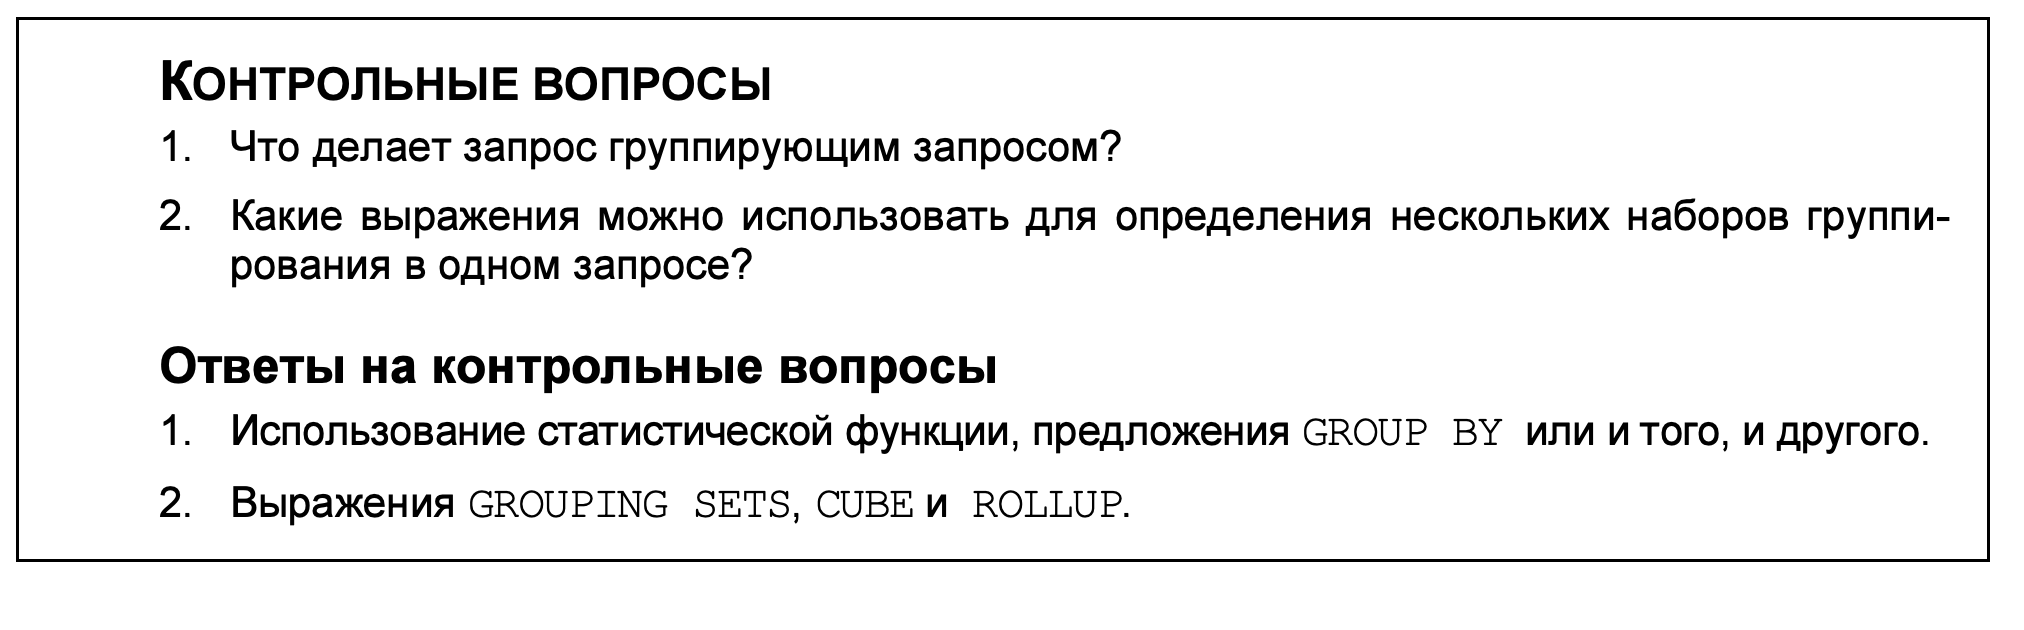
\includegraphics[width=0.8\textwidth]{img/control14.png}
	\end{center}
	\captionsetup{justification=centering}
\end{figure}	


\subsection*{Резюме занятия}
\begin{itemize}
	\item Язык T-SQL позволяет группировать данные и выполнять операции анализа
	данных на группах. 
	\item Можно применять статистические функции, такие как COUNT, SUM, AVG, MIN и MAX,
	к группам. 
	\item Стандартные групповые запросы определяют только один набор группирования. 
	\item Новую функциональность языка T-SQL можно использовать для определения
	нескольких наборов группирования в одном запросе с помощью выражений
	GROUPING SETS, CUBE и ROLLUP.  
\end{itemize}

\subsection*{Закрепление материала}

\begin{figure}[h!]
	\begin{center}
		
\includegraphics[width=0.9\textwidth]{img/zakrep11.png}
	\end{center}
	\captionsetup{justification=centering}
\end{figure}
\newpage

\subsection*{Ответы}

\begin{figure}[h!]
	\begin{center}
		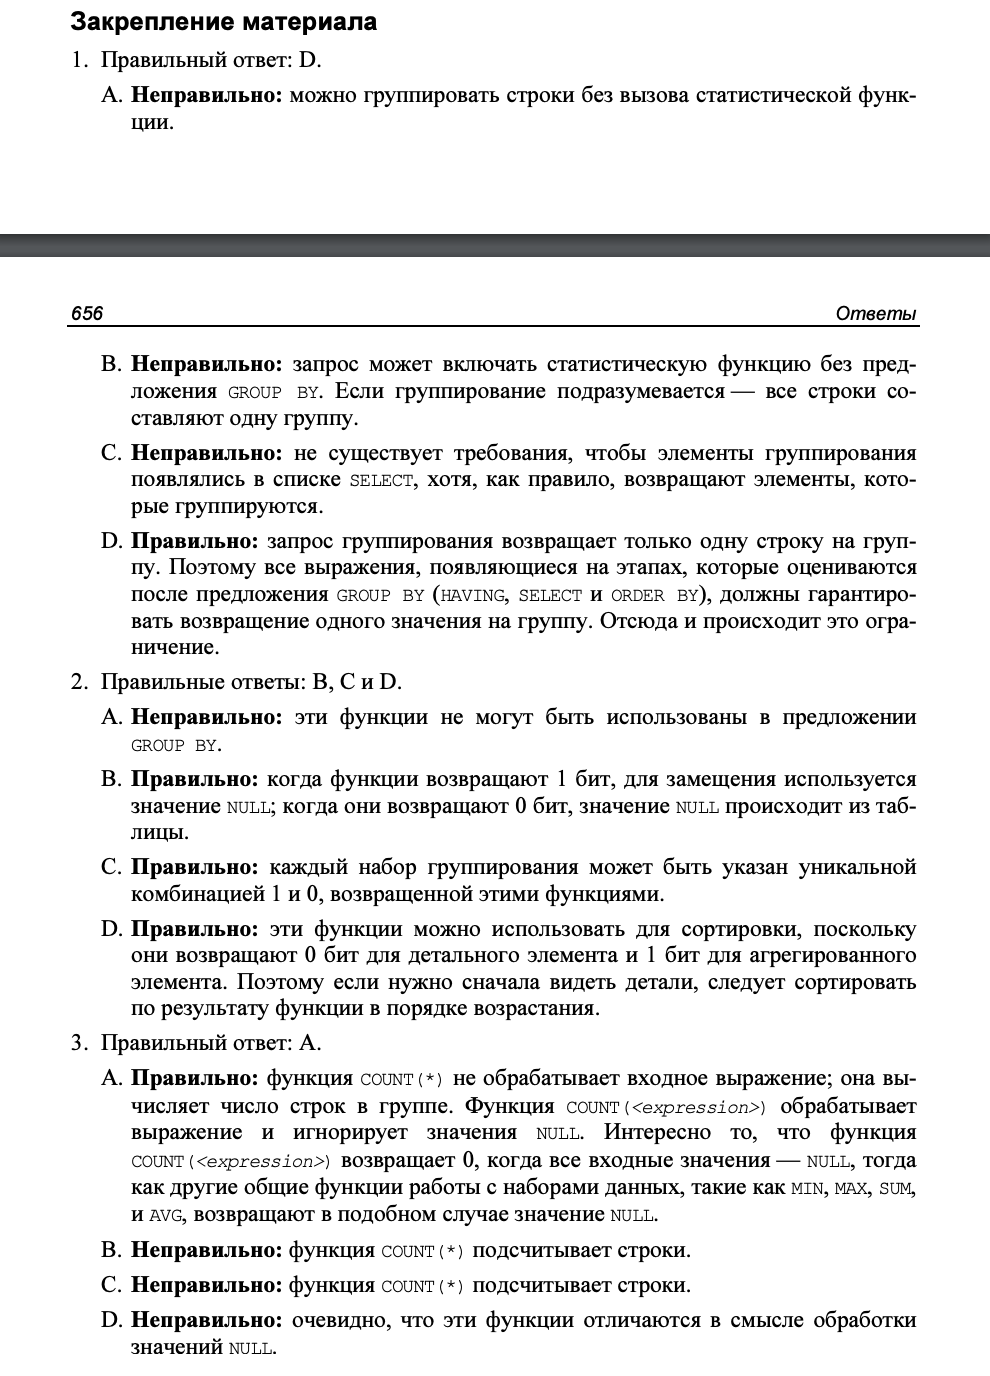
\includegraphics[width=0.9\textwidth]{img/ans11.png}
	\end{center}
	\captionsetup{justification=centering}
\end{figure}
\clearpage


\section{Сведение и отмена сведения данных}

\subsection{Сведение данных}

Сведение — это технология группирования и агрегирования данных путем трансформации их из состояния строк в состояние столбцов. Во всех запросах сведения
необходимо указать три элемента:

\begin{itemize}
	\item Что вы хотите видеть в строках? Этот элемент называется on rows, или
	группирующий элемент (grouping element). 
	\item Что вы хотите видеть в столбцах? Этот элемент называется on cols, или распределяющий элемент (spreading element).
	\item Что вы хотите видеть на пересечении каждого отдельного значения строки и
	столбца? Этот элемент известен как данные (data), или агрегатный элемент
	(aggregation element). 
\end{itemize}


\begin{lstlisting}[label=lst:funcReturn, language=sql]
	WITH PivotData AS
( SELECT
 <grouping column>,
 <spreading column>,
 <aggregation column>
 FROM <source table>
)
SELECT <select list>
FROM PivotData
 PIVOT(<aggregate function>(<aggregation column>)
 FOR <spreading column> IN (<distinct spreading values>)) AS P; 
\end{lstlisting}	


\begin{lstlisting}[label=lst:funcReturn, caption=Вывод суммы заказа у каждого поставщика, language=sql]
WITH PivotData AS
( SELECT
	custid, 
	shipperid, 
	freight 
	FROM Sales.Orders )
SELECT custid, [1], [2], [3]
FROM PivotData
PIVOT(SUM(freight) FOR shipperid IN ([1],[2],[3]) ) AS P; 
\end{lstlisting}


\subsection{Отмена сведения данных}
При отмене
сведения данных входные данные разворачиваются из состояния столбцов в состояние строк.

Помните, в каждой задаче отмены сведения необходимо указать следующие три элемента: 

\begin{itemize}
	\item набор исходных столбцов, для которых нужно выполнить отмену сведения
	(в данном случае [1], [2], [3]); 
	\item имя, которое будет присвоено столбцу с полученными значениями (в данном
	случае freight); 
	\item имя, которое вы хотите присвоить столбцу целевых имен (в данном случае
	shipperid). 
\end{itemize}

\begin{lstlisting}[label=lst:funcReturn,  language=sql]
	SELECT <column list>, <names column>, <values column>
	FROM <source table>
	UNPIVOT(<values column> FOR <names column> IN(<source columns>)) AS U; 
\end{lstlisting}

\begin{lstlisting}[label=lst:funcReturn, language=sql]
	SELECT custid, shipperid, freight
	FROM Sales.FreightTotals
	UNPIVOT(freight FOR shipperid IN([1],[2],[3])) AS U; 
\end{lstlisting}


\begin{figure}[h!]
	\begin{center}
		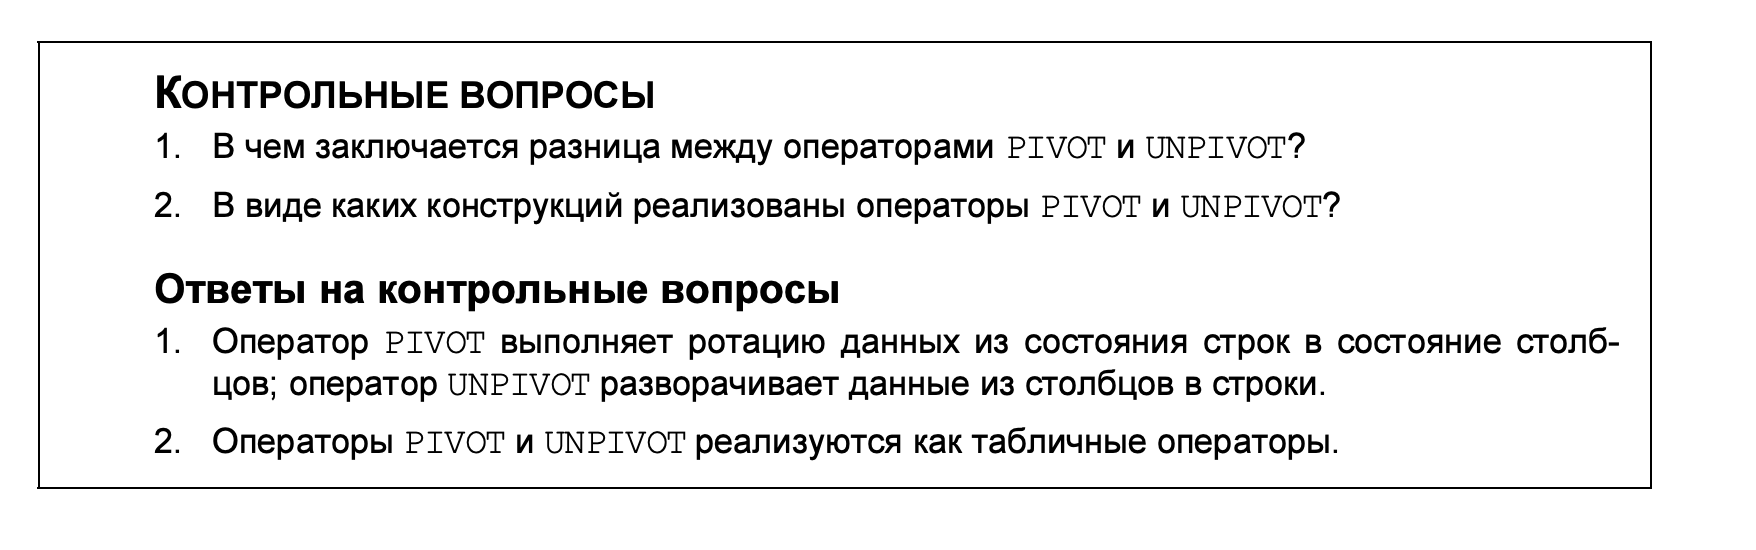
\includegraphics[width=0.9\textwidth]{img/control15.png}
	\end{center}
	\captionsetup{justification=centering}
\end{figure}
		
\subsection*{Резюме занятия}
\begin{itemize}
	\item Сведение данных — это особая форма группирования и агрегирования данных,
	когда данные разворачиваются из состояния строк в состояние столбцов. 
	\item При сведении данных необходимо указать три вещи: группирующий элемент,
	распределяющий элемент и агрегатный элемент. 
	\item T-SQL поддерживает собственный оператор PIVOT, используемый для сведения
	данных входной таблицы. 
	\item Отмена сведения данных трансформирует данные из состояния столбцов в состояние строк. 
	\item Чтобы выполнить отмену сведения данных, необходимо указать три вещи: исходные столбцы, для которых нужно выполнить отмену сведения, столбец целевых имен и столбец целевых значений. 
	\item T-SQL поддерживает собственный оператор с именем UNPIVOT, который применяется для отмены сведения данных входной таблицы. 
\end{itemize}


\subsection*{Закрепление материала}

\begin{figure}[h!]
	\begin{center}
		
\includegraphics[width=0.9\textwidth]{img/zakrep12.png}
	\end{center}
	\captionsetup{justification=centering}
\end{figure}
\clearpage

\subsection*{Ответы}

\begin{figure}[h!]
	\begin{center}
		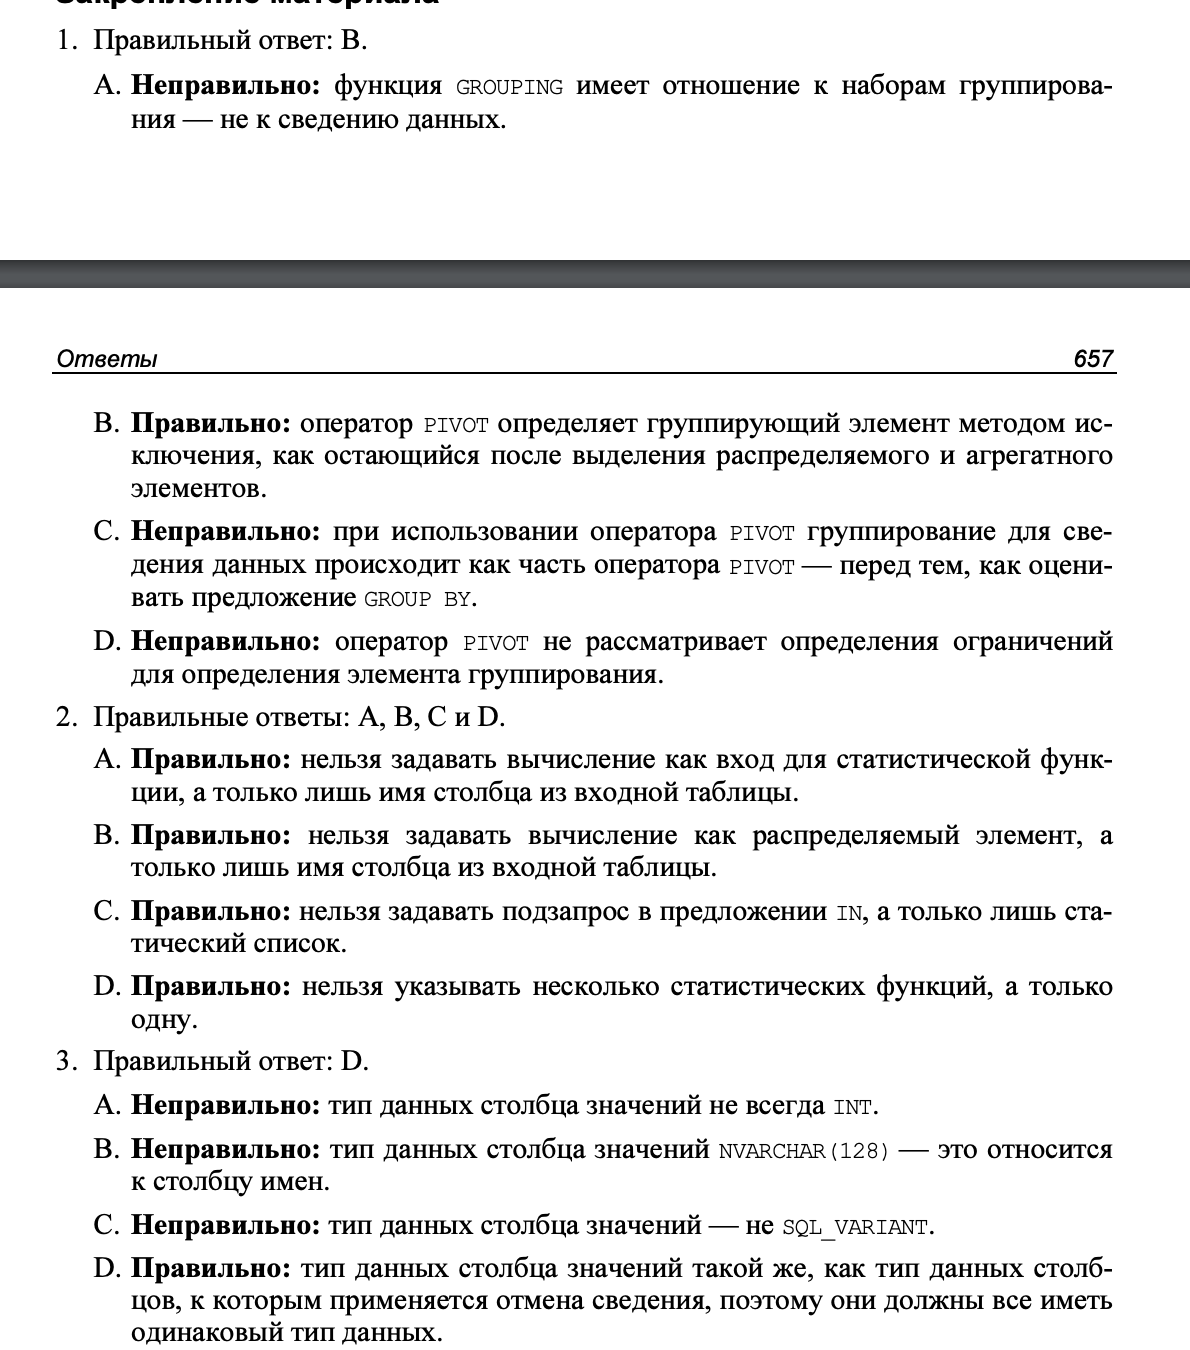
\includegraphics[width=0.9\textwidth]{img/ans12.png}
	\end{center}
	\captionsetup{justification=centering}
\end{figure}


\section{Использование оконных функций}

\subsection{Статистические оконные функции}

Следующий запрос вычисляет для каждого заказа процент стоимости текущего заказа от суммарной стоимости по клиенту, а
также процент от полной стоимости. 


\begin{lstlisting}[label=lst:funcReturn, language=sql]
	SELECT custid, orderid, val,
	CAST(100.0 * val / SUM(val) OVER(PARTITION BY custid) AS NUMERIC(5, 2)) AS
   pctcust,
	CAST(100.0 * val / SUM(val) OVER() AS NUMERIC(5, 2)) AS pcttotal
   FROM Sales.OrderValues;
\end{lstlisting}

Оконные агрегатные функции поддерживают еще одну возможность фильтрации,
называемую кадрированием. Смысл ее заключается в том, что определяется упорядочение внутри секции с помощью предложения оконного кадра и затем, на основе
этого упорядочения, можно заключить набор строк между двумя границами.

В предложении оконного кадра указываются единицы измерения (ROWS или RANGE) и
экстент оконного кадра (смещение границ по отношению к текущей строке). Используя предложение ROWS, можно указать границы как один из следующих параметров:

\begin{itemize}
	\item UNBOUNDED PRECEDING или FOLLOWING, означающие начало или конец секции соответственно; 
	\item CURRENT ROW, представляющий текущую строку;
	\item <n> ROWS PRECEDING или FOLLOWING, означающие n строк перед или после текущей
	строки соответственно. 
\end{itemize}

Пусть вам нужно отфильтровать результат запроса, возвратив только те
строки, в которых промежуточная сумма меньше 1000,00. Следующий код решает
эту задачу путем определения обобщенного табличного выражения (common table
expression, CTE), используя предыдущий запрос и затем выполняя фильтрацию во
внешнем запросе. 

\begin{lstlisting}[label=lst:funcReturn, language=sql]
	WITH RunningTotals AS
	( SELECT custid, orderid, orderdate, val,
	 SUM(val) OVER(PARTITION BY custid
	 ORDER BY orderdate, orderid
	 ROWS BETWEEN UNBOUNDED PRECEDING
	 AND CURRENT ROW) AS runningtotal
	 FROM Sales.OrderValues )
	SELECT *
	FROM RunningTotals
	WHERE runningtotal < 1000.00; 
\end{lstlisting}

Еще один пример ограничителя оконного кадра: если было бы нужно, чтобы кадр
включал только последние 3 строки, следовало бы использовать формат ROWS
BETWEEN 2 PRECEDING AND CURRENT ROW. 

Что касается ограничителя оконного кадра RANGE, согласно стандартному языку
SQL, он позволяет определять ограничители на основе логических смещений от
ключа сортировки текущей строки. 

Помните, что предложение ROWS определяет  ограничители — число строк от текущей строки, — на основе физических смещений.


\begin{figure}[h!]
	\begin{center}
		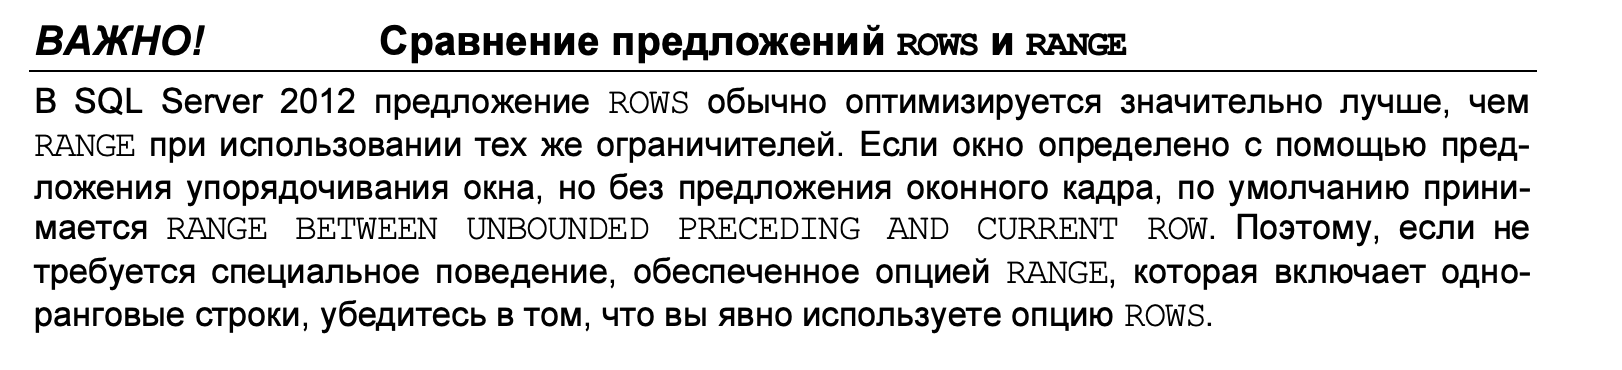
\includegraphics[width=0.9\textwidth]{img/warn2.png}
	\end{center}
	\captionsetup{justification=centering}
\end{figure}


\subsection{Ранжирующие оконные функции}

T-SQL поддерживает четыре ранжирующие оконные
функции: ROW\_NUMBER, RANK, DENSE\_RANK и NTILE.

Следующий запрос демонстрирует использование этих функций. 

\begin{lstlisting}[label=lst:funcReturn, language=sql]
	SELECT custid, orderid, val,
	ROW_NUMBER() OVER(ORDER BY val) AS rownum,
	RANK() OVER(ORDER BY val) AS rnk,
	DENSE_RANK() OVER(ORDER BY val) AS densernk,
	NTILE(100) OVER(ORDER BY val) AS ntile100
   FROM Sales.OrderValues; 
\end{lstlisting}
	
Этот запрос генерирует следующий результат (показанный здесь в сокращенном
виде): 

\begin{figure}[h!]
	\begin{center}
		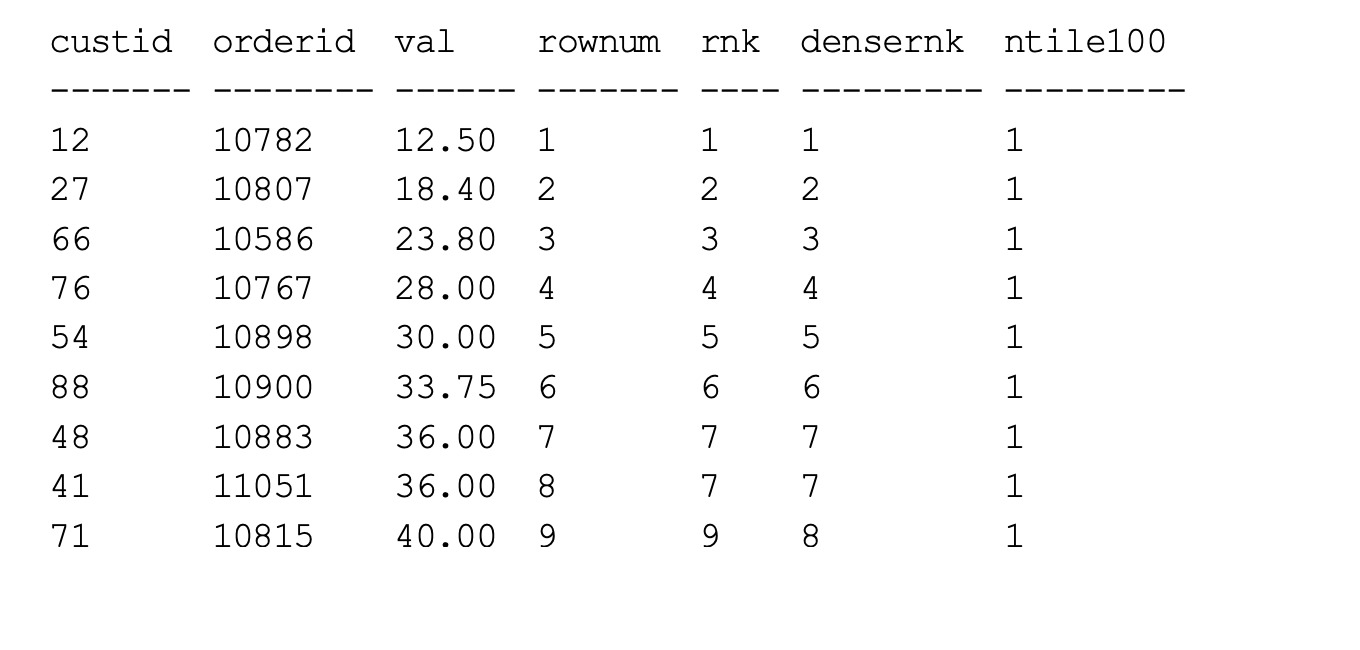
\includegraphics[width=0.9\textwidth]{img/res15.png}
	\end{center}
	\captionsetup{justification=centering}
\end{figure}


\begin{figure}[h!]
	\begin{center}
		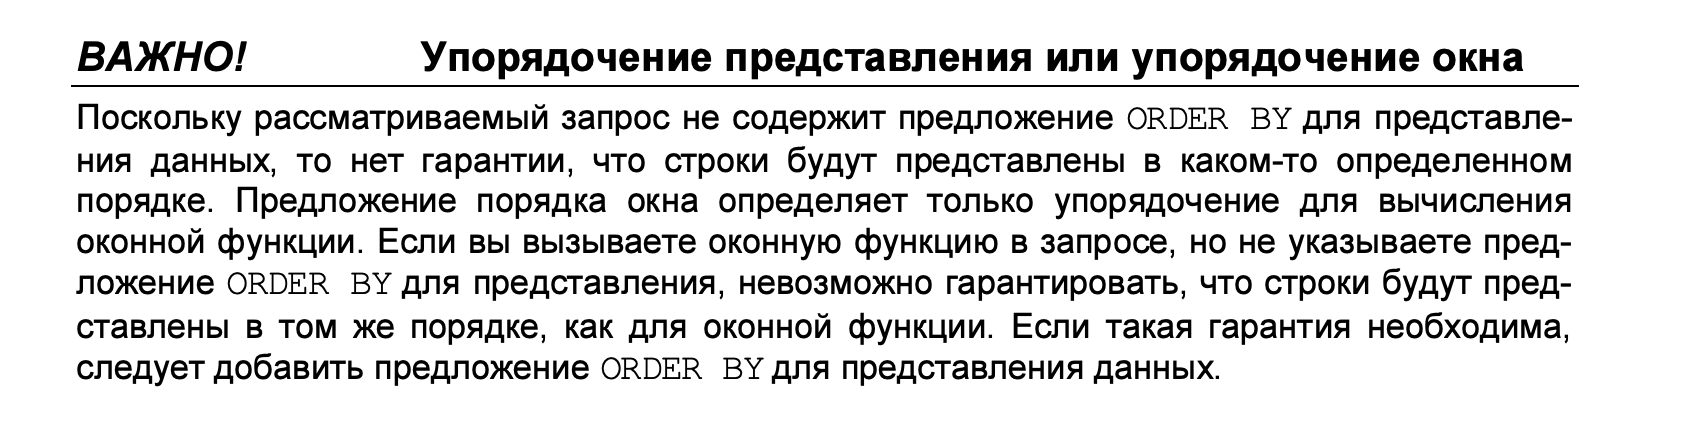
\includegraphics[width=0.9\textwidth]{img/warn3.png}
	\end{center}
	\captionsetup{justification=centering}
\end{figure}


Функция ROW\_NUMBER вычисляет уникальный последовательный номер строки, начиная с 1, в секции окна на основании сортировки окна. Поскольку рассматриваемый
в примере запрос не содержит предложение секционирования окна, эта функция
рассматривает результирующий набор как одну секцию; следовательно, функция
присваивает уникальные номера строк для всего результирующего набора запроса. 

Функция RANK возвращает число строк в секции,
которые имеют более низкое значение сортируемого столбца, чем текущее, плюс 1. 

Функция DENSE\_RANK возвращает количество предшествующих отличающихся значений упорядочиваемого столбца с более низким значением, чем текущее, плюс 1. 

Функция NTILE позволяет организовать строки внутри секции в запрашиваемое количество групп одинакового размера на основе указанной сортировки.

\begin{figure}[h!]
	\begin{center}
		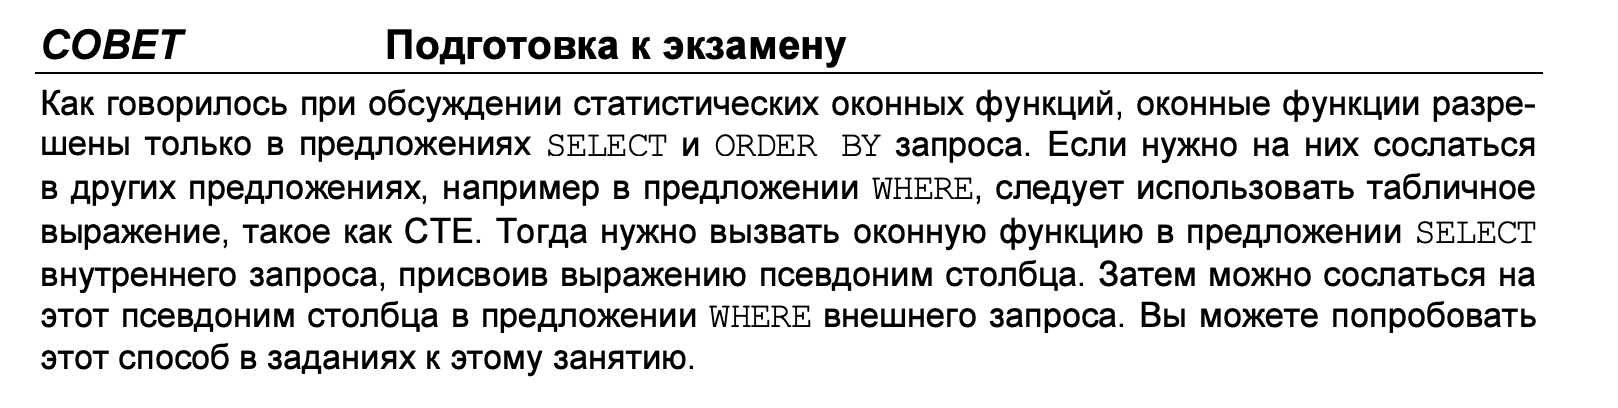
\includegraphics[width=0.9\textwidth]{img/advice10.png}
	\end{center}
	\captionsetup{justification=centering}
\end{figure}


\subsection{Оконные функции смещения}

Оконные функции смещения возвращают элемент строки, которая находится на
указанном смещении от текущей строки в секции окна или от первой либо последней строки оконного кадра. T-SQL поддерживает следующие оконные функции
смещения: LAG, LEAD, FIRST\_VALUE и LAST\_VALUE.

Функции LAG и LEAD используют смещение относительно текущей строки, а функции FIRST\_VALUE и LAST\_VALUE работают с первой или последней строкой окна соответственно. 

Функция LAG возвращает элемент строки в текущей секции, который является запрашиваемым числом
строк перед данной строкой (на основании сортировки окна), при этом смещение
по умолчанию принимается равным 1. Функция LEAD возвращает элемент строки,
который находится на запрашиваемом смещении после текущей строки. 


\begin{lstlisting}[label=lst:funcReturn, language=sql]
	SELECT custid, orderid, orderdate, val,
	LAG(val) OVER(PARTITION BY custid
	ORDER BY orderdate, orderid) AS prev_val,
	LEAD(val) OVER(PARTITION BY custid
	ORDER BY orderdate, orderid) AS next_val
   FROM Sales.OrderValues; 
\end{lstlisting}

\begin{figure}[h!]
	\begin{center}
		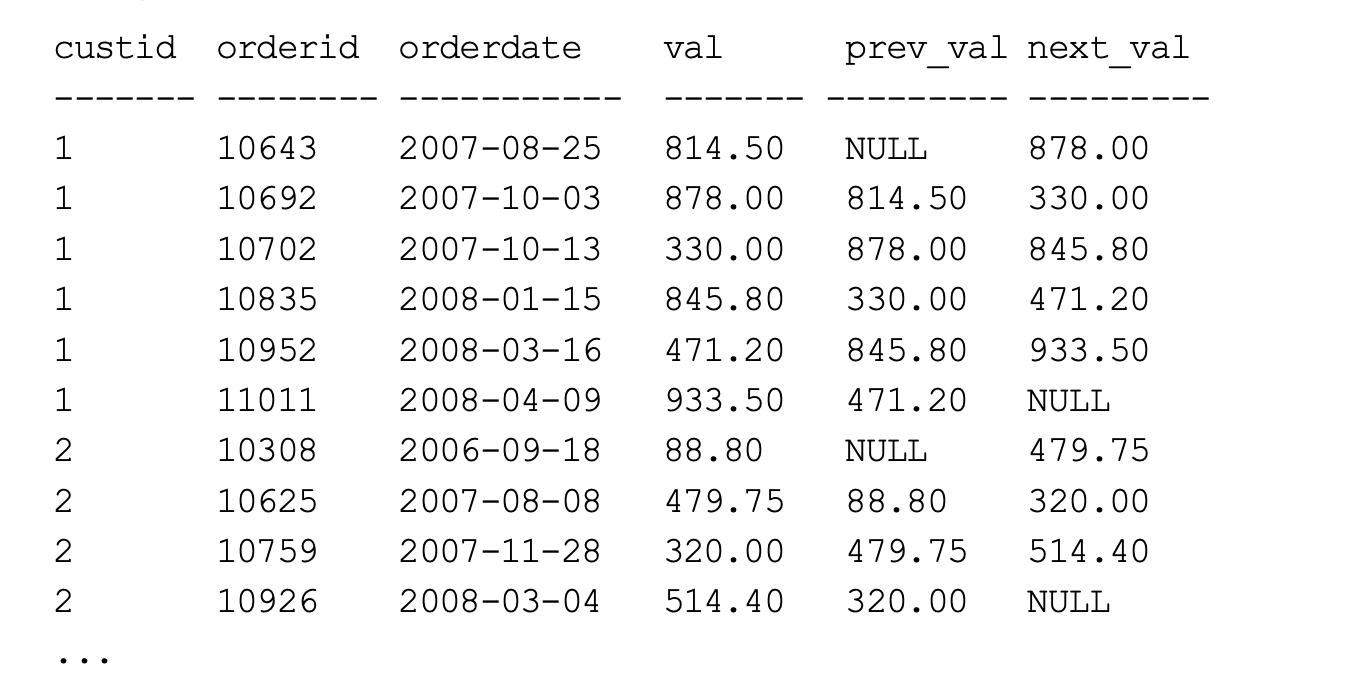
\includegraphics[width=0.9\textwidth]{img/res10.png}
	\end{center}
	\captionsetup{justification=centering}
\end{figure}

При желании иметь смещение, отличное от 1,
следует указать его вторым аргументом, как в случае LAG(val, 3). 

Заметьте, что если строка не существует на запрашиваемом смещении, функция
возвращает по умолчанию значение NULL. Если в этом случае нужно возвращать
другое значение, его следует указать в качестве третьего элемента, как в случае
LAG(val, 3, 0). 


\begin{figure}[h!]
	\begin{center}
		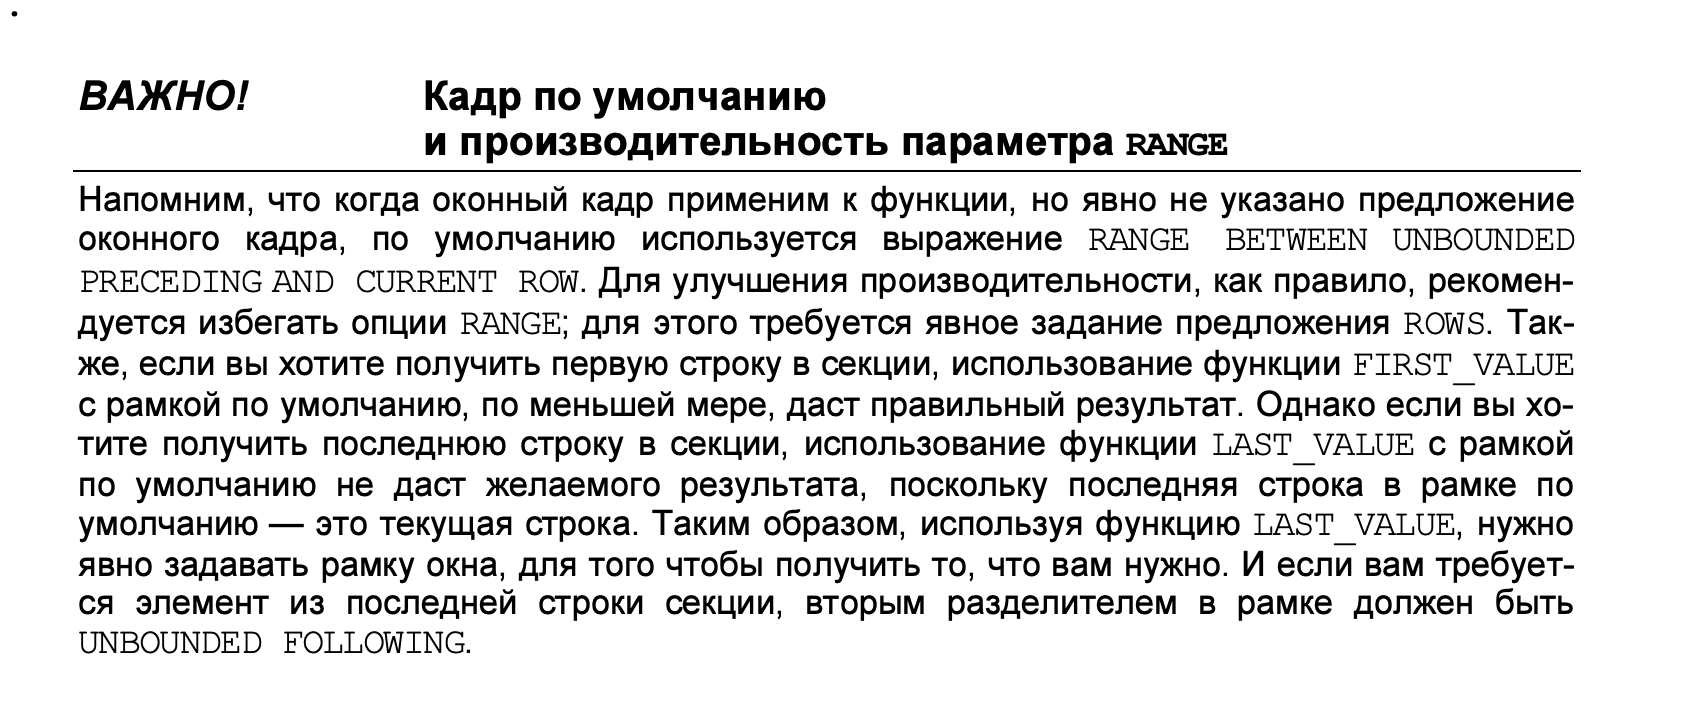
\includegraphics[width=0.9\textwidth]{img/warn4.png}
	\end{center}
	\captionsetup{justification=centering}
\end{figure}


\begin{figure}[h!]
	\begin{center}
		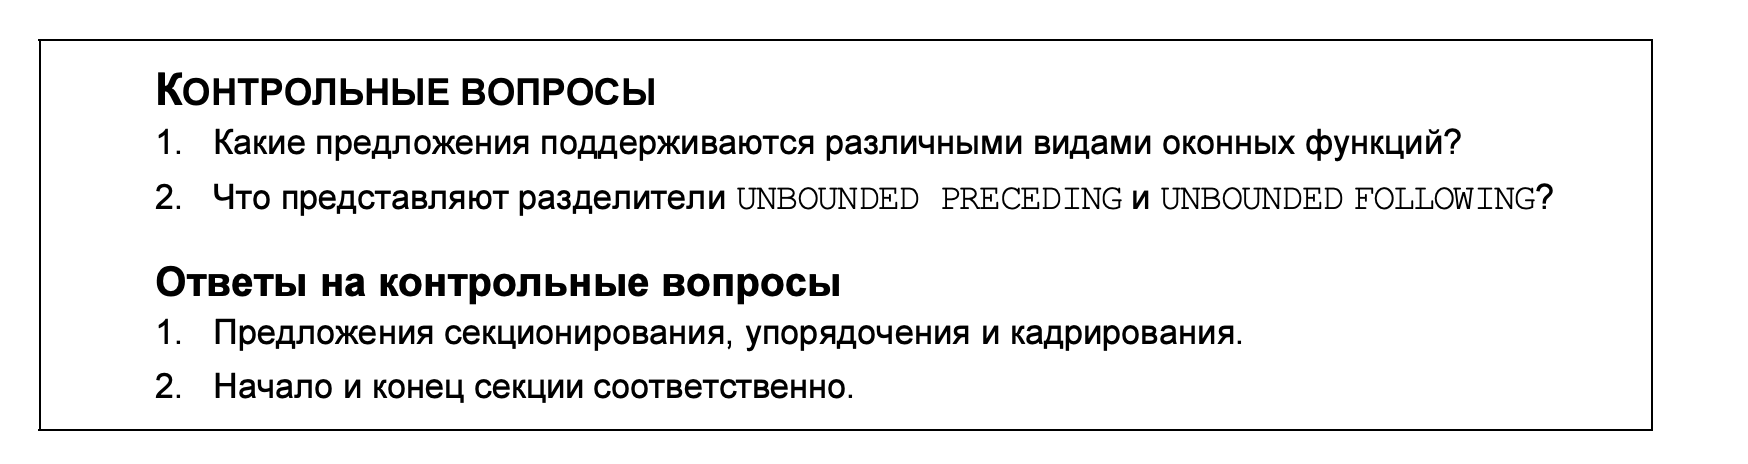
\includegraphics[width=0.9\textwidth]{img/control16.png}
	\end{center}
	\captionsetup{justification=centering}
\end{figure}



\subsection*{Резюме занятия}
\begin{itemize}
	\item Оконные функции выполняют аналитические вычисления данных. Они обрабатывают набор строк, определенный для каждой базовой строки, с помощью
	предложения OVER. 
	\item Язык T-SQL поддерживает статистические, ранжирующие оконные функции,
	а также оконные функции смещения. Все оконные функции поддерживают
	предложения секционирования и сортировки. Статистические оконные функции, кроме FIRST\_VALUE и LAST\_VALUE, также поддерживают предложение оконного кадра. 
	\item В отличие от группирующих запросов, которые скрывают строки детализации и
	возвращают только одну строку на группу, оконные запросы не скрывают эти
	строки. Они возвращают одну строку на каждую строку в базовом запросе и позволяют смешивать элементы детализации и оконные функции в одних и тех же
	выражениях. 
\end{itemize}

\subsection*{Закрепление материала}

\begin{figure}[h!]
	\begin{center}
		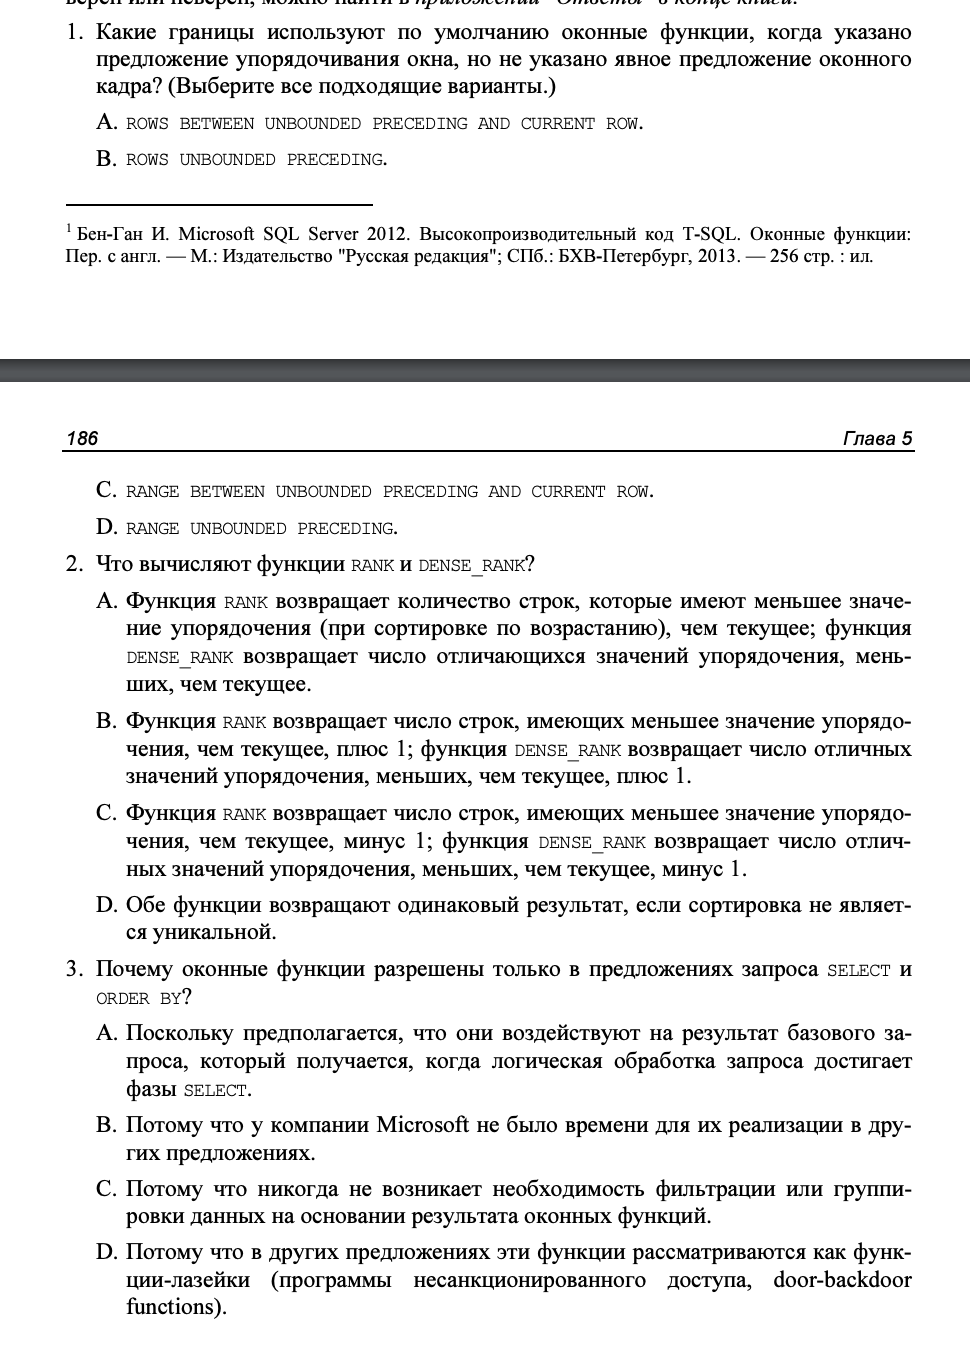
\includegraphics[width=0.9\textwidth]{img/zakrep13.png}
	\end{center}
	\captionsetup{justification=centering}
\end{figure}
\clearpage

\subsection*{Ответы}

\begin{figure}[h!]
	\begin{center}
		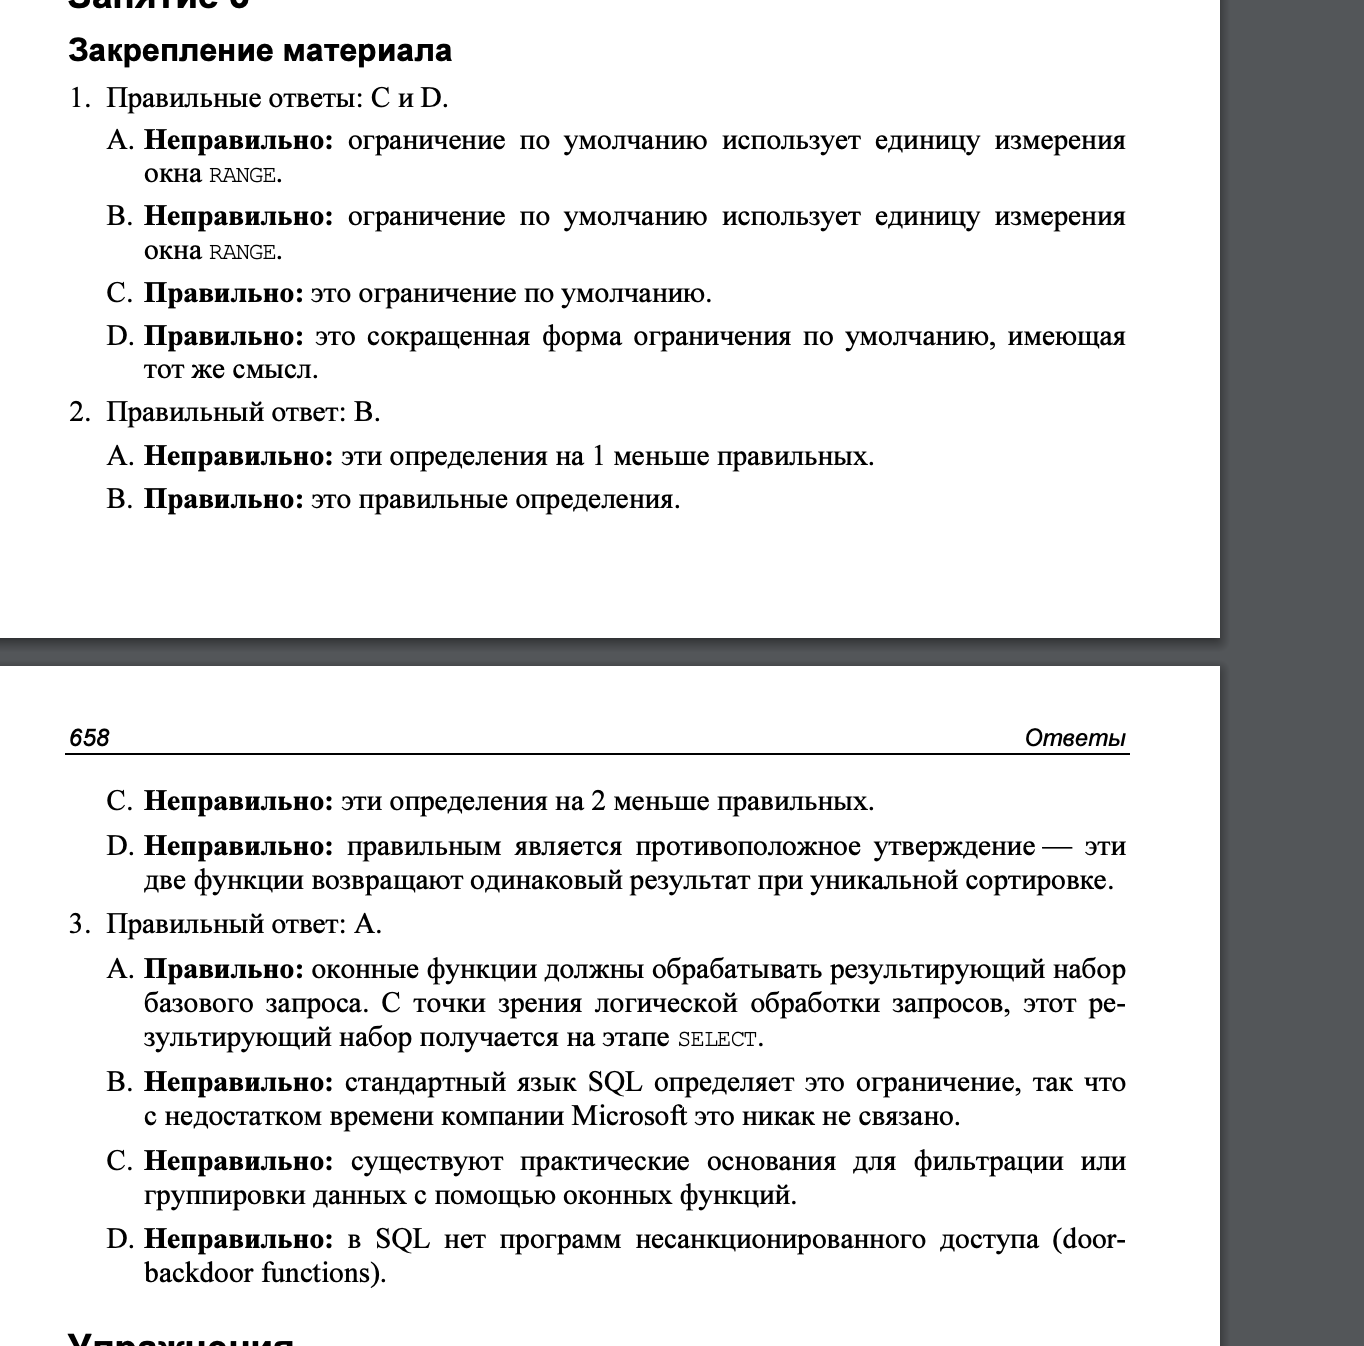
\includegraphics[width=0.8\textwidth]{img/ans13.png}
	\end{center}
	\captionsetup{justification=centering}
\end{figure}



\newpage
\subsection*{Упражнения}

\begin{figure}[h!]
	\begin{center}
		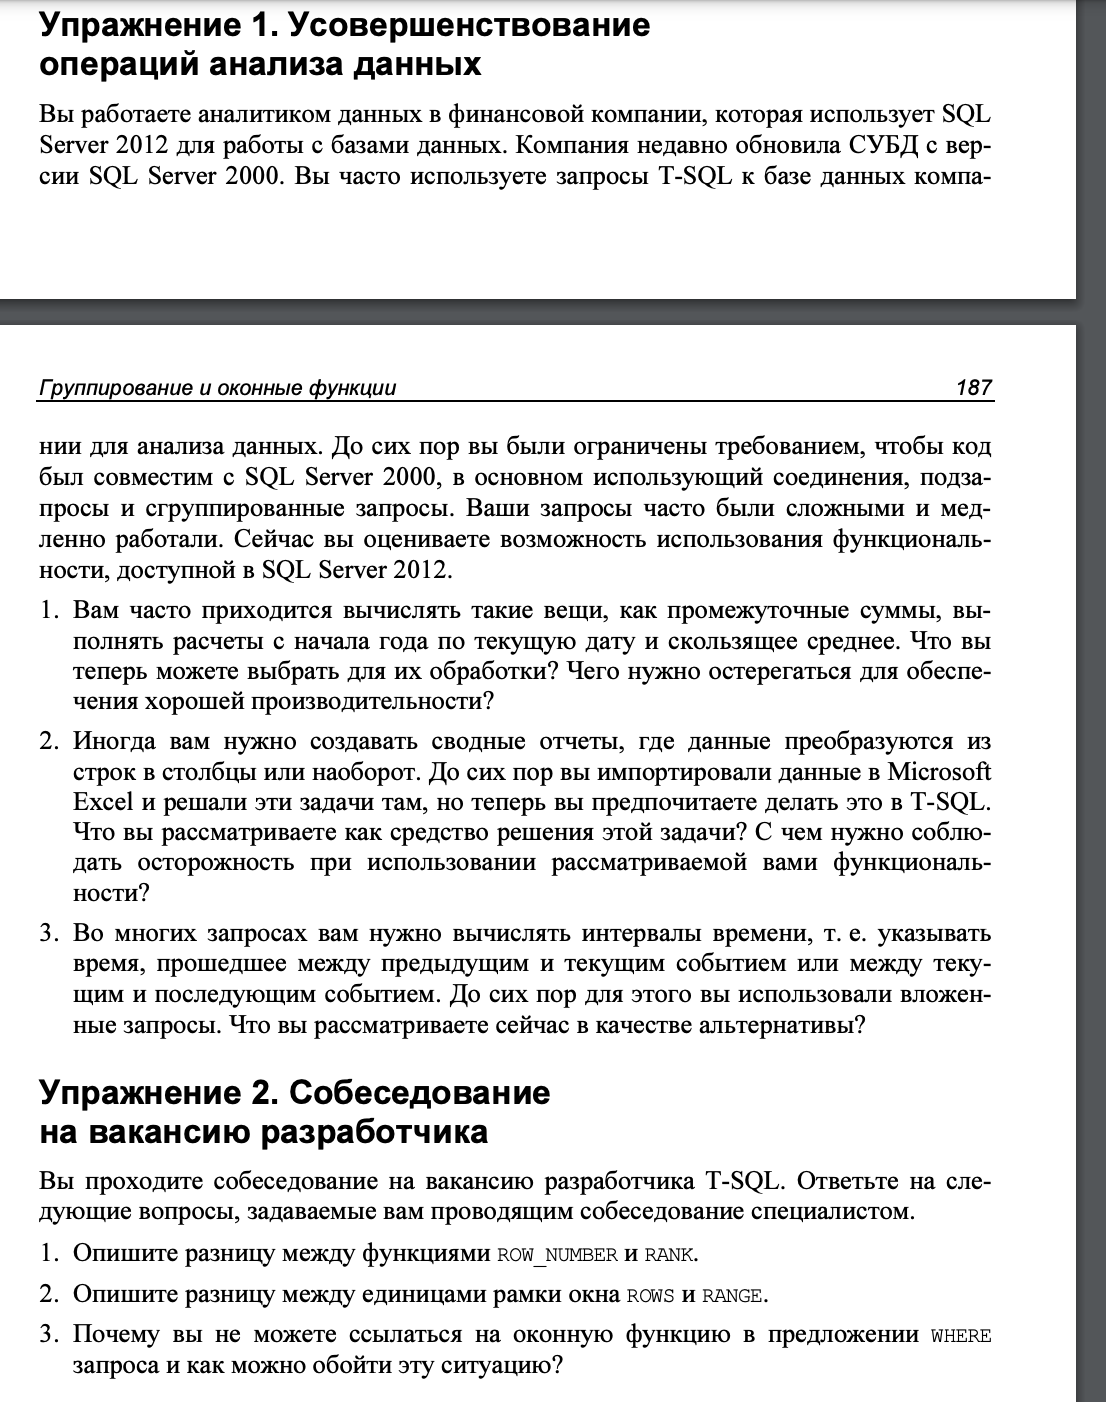
\includegraphics[width=0.9\textwidth]{img/ex13.png}
	\end{center}
	\captionsetup{justification=centering}
\end{figure}

\subsection*{Ответы}

\begin{figure}[h!]
	\begin{center}
		
\includegraphics[width=0.9\textwidth]{img/ans14.png}
	\end{center}
	\captionsetup{justification=centering}
\end{figure}





